% !TEX root = ./HY-CS-main.tex
\color{black}
\chapter{Datamalli oppijan kehittymisestä\label{datamallioppijankehittymisesta}}

\color{blue}
Oppimisanalytiikassa yhdistelemällä tilastollisia menetelmiä ja ennustavaa mallintamista voidaan kohdentaa ohjausta oppijoiden haasteisiin oppimisessa ja tarjoamalla kohdistettua tukea saatavan datan avulla \citep{ranjeethSurveyPredictiveModels2020}. Käytettävät ennustavat mallit voivat olla mitä vain datanlouhinta-, koneoppimis- ja keinoälymenetelmiä. Datalähteenä malleille voidaan hyödyntää eri oppijasta tietoa sisältäviä järjestelmiä, kuten verkko-oppimisympäristö Moodlea.
% Huomioi myös Moodle datalähteenä ingressiin.
\color{black}

\section{Moodle datalähteenä}

Moodle (Modular Object-Oriented Dynamic Learning System) on vuodesta 1999 lähtien kehittetty avoimen lähdekoodin verkko-oppimisympäristö, joka on julkaistu GPL-3.0 -lisenssillä \citep{dougiamasPowerOpenEducational2021,dougiamasMoodle2022}. Moodlella on yli 315 miljoonaa käyttäjää eri puolilla maailmaa 178 tuhannella eri Moodle-sivustolla \citep{moodle.orgMoodleStatistics}. Moodle on rakennettu käyttäen ohjelmointikielenä PHP:tä ja tiedon tallentamiseen relaatiotietokantaa. Suorat SQL-kyselyt tietokantaan ja Moodlen tarjoamat metodit mahdollistavat Moodlen keräämän tiedon hyödyntämisen osana data-analyysia. Moodlen tietokantarakenteesta löytyy selkeä indeksointi avaimien perusteella \citep{greenMoodle11Database2022}, jonka perusteella tietokantataulusta toiseen asioiden jäljittäminen on mahdollista.

Moodlessa on vakiona 23 erilaista aktiviteettiä, joista jokainen tallentaa erilaista tietoa tietokantaan \citep{dougiamasMoodle2022}. Jokaisella aktiviteetillä on myös omia tietokantatauluja, joihin tallennetaan aktiviteettiin liittyvä tieto. Lisäksi Moodlen kehittäjäyhteisö on julkaissut paljon Moodlea laajentavia aktiveettejä \citep{moodle.orgMoodlePluginsDirectory2022}. Oppilaan osaamista mittaavia aktiviteettejä ovat esimerkiksi tentti, palaute, työpaja, oppitunti, keskustelualue ja H5P. Esimerkiksi työpaja tallentaa kaikki suoritukset tauluun \emph{workshop\_submissions} ja suorituksien arvioinnit tauluun \emph{workshop\_grades} \citep{greenMoodle11Database2022}. Työpaja mahdollistaa myös vertaisarvioinnin (taulussa \emph{workshop\_assessments}), jossa oppija joutuu arvioimaan omaa ja toisten osaamista hyödyntämisen analytiikassa. Keskustelualueelta voidaan mitata oppijoiden aktiivisuutta viestien lukumäärällä \citep{mwalumbweUsingLearningAnalytics2017}. Aktiviteetistä myös saadaan tieto, onko sitä avattu kertaakaan taulusta \emph{course\_module\_completion}.

Moodle tallentaa tietokantatauluun \emph{logstore\_standard\_log} kaikki Moodlen Event API:n kautta tulevat tapahtumat \citep{dougiamasMoodle2022, dougiamasLoggingMoodleDocs2021}. Tapahtumien avulla voidaan kerätä tietoa toiminnasta verkko-oppimisympäristössä \citep{agudo-peregrinaCanWePredict2014}. Lokitietoa erilaisista tapahtumista voi esimerkiksi tulla Moodlen ytimen komponenteista, eri aktiviteeteistä, työkaluista ja raporteista riippuen komponentin luonteesta. Useimmat aktiviteetit tallentavat lokiin merkittäviä tapahtumia, kuten suorituksien luomisen aktiviteettiin, kurssimoduulissa vierailun, tenttiin vastaamisen ja vertaisarvioinnin antamisen. Moodlen ytimessä oppijan kannalta tärkeimmät ovat kirjautumiseen ja kurssin katseluun liittyvät tapahtumat. Lokitietoihin tallentuu aina tieto kuka on vieraillut, milloin on vieraillut, missä on vieraillut ja mistä on vieraillut \citep{abdullahLearningStyleClassification2015}. Tapahtumalokin avulla voidaan tarkastella oppijoiden toiminnan painottumista eri kellonaikoihin.

Moodlen yhteisö on myös etsinyt erilaisia tapoja kerätä palautetta oppijoilta. Yksi tälläinen on pikapalautetoiminnallisuus (block\_point\_view), joka antaa kolmiportaisen itsearviointimahdollisuuden aktiviteettikohtaisesti \citep{fombaronMoodlePluginPoint2021}. Tämä mahdollistaa helpon ja nopean tavan saada oppijalta itsearviointidataa siitä, miten oppija itse näkee oman suoriutumisensa kyseisessä tehtävässä. Tietokantataulusta \emph{block\_point\_view} pystytään hakemaan käyttäjän äänestystulos kurssin, kurssimoduulin tai käyttäjän perusteella.

Joidenkin tietojen, kuten oppijan tarkemman toiminnan seuraamiseen sivulla tarvitaan kolmannen osapuolen tuottamaa tekniikkaa \citep{filvaGoogleAnalyticsTime2014}. Tälläinen seuraamiseen soveltuva työkalu on esimerkiksi Google Analytics, joka seuraa tarkemmin käyttäjän toimintaa sivustolla. Moodlen lokitiedoista selviää milloin sivu on ladattu, mutta tietoa kuinka kauan oppija sivulla on todellisuudessa viettänyt aikaa ei tällä menetelmällä saada \citep{dougiamasMoodle2022}. On teoreettisesti mahdollista, että oppija on avattuaan sivun katsellut sitä minuutin ajan ja tämän jälkeen lähtenyt kahville. Jos seuraava sivulataus on tunnin päästä, niin tästä ei pystytä luotettavasti laskemaan sivulla vietettyä todellista aikaa.

\color{blue}
Learning Analytics API tarjoaa Moodlen oman rajapinnan oppimisanalytiikan toteuttamiseen \citep{oliveSupervisedLearningFramework2018}. Moodlessa se jakautuu kahteen osaan, Moodlen Analytics API:n ja Machine Learning backendiin. Analytics API tuottaa mallien tarvitsemaa tietoa koneluettavassa CSV-muodossa. Backend puolestaan vastaa itse tiedon käsittelystä ja analysoinnista.
\color{black}

\section{Yleistetty malli}
\color{red}
tilastollinen malli kuvaa optimia, ja verrataan kuinka data sopii tähän malliin
\color{black}

% Linear regressionista hyvää tietoa \citep{rossIntroductoryStatistics2017} - Ch 12 \\
% Naive Bayessian Ch 16
Datamallin rakentaminen on iteratiivinen prosessi, jossa on useita vaiheita \citep{hamalainenClassifiersEducationalData2010}. Iteratiivisen prosessin aikana kokeillaan useita erilaisia malleja, datan esitysmuotoja ja algoritmien asetuksia löytääksemme parhaan mahdollisen datamallin. Valitun mallin toimivuus voidaan todentaa luokittelun onnistumisella, sillä mallin soveltuvuus voidaan kyseenalaistaa liian monen luokitteluvirheen jälkeen.

% HOX TÄÄ TARVII UUDELLEENKIRJOITUSTA, MUTTA MITEN!?
Oppimisanalytiikassa usein käytetään luokittelua, jota hyödynnetään opetuksessa yleisesti opettajien arvioidessa oppijoiden tietotasoa, motivaatiota ja käytöstä \citep{hamalainenClassifiersEducationalData2010}. Oppimisanalytiikassa luokittelua tehdään selitettävän muuttujan arvoa ennustavalla mallilla, jota ennustetaan selittävien muuttujien arvojen avulla. Luokittimia voidaan tehdä joko ammattilaisten käsityönä tai nykyisin yleisemmällä tavalla opettaa luokitin luokittelemaan olemassa olevalla datalla.

Useissa oppimisanalytiikkaa käsittelevissä tutkimuksissa on kokeiltu erilaisia luokittelualgoritmejä parhaiten toimivan mallin löytämiseksi \citep{akcapinarUsingLearningAnalytics2019}. Usein käytettyjä algoritmejä ovat naiivi Bayes, Classification Tree, Random Forest, tukivektorikone (SVM), neuroverkko, CN2 rules ja k-lähinaapurimenetelmä. Yksi tapa etsiä parhaiten toimivaa mallia on tehdä suorituskykymittauksia, joissa tarkastellaan tarkkuutta, herkkyyttä, yksityiskohtaisuutta ja F-Measurea.

Yksi tapa tehdä luokittelua on käyttää naiivia Bayesin luokitinta \citep{natinggaDataScienceAlgorithms2018}. Naiivi Bayesin luokitin pohjautuu Bayesin teoreemaan $$P(A | B) = \frac{P(B | A) \cdot P(A)}{P(B)},$$ missä $A$ ja $B$ ovat tapahtumia, $P(A)$ on todennäköisyys tapahtumalle $A$ olla tosi ja $P(A | B)$ on ehdollinen todennäköisyys tapahtumalle $A$ olla tosi, mikäli tapahtuma $B$ on tosi. Naiivissa Bayesin luokittimessa datapisteiden joukolle annetaan Bayesin teoreeman perusteella todennäköisin luokka. Tämä tapahtuu laskemalla todennäköisyys sille, kuinka todennäköisesti asia A tapahtuu, jos ehto B saa tietyn arvon.

Bayesin teoreemaa voidaan hyödyntää myös useamman todennäköisyystapahtuman kanssa, jolloin käytetään laajennettua Bayesin teoreemaa \citep{natinggaDataScienceAlgorithms2018}. Jos määritellään tapahtumat $B_1, \ldots, B_n$ olemaan ehdollisesti riippumattomia tapahtumasta $A$, niin Bayesin teoreema voidaan esittää muodossa $$P(A | B_1, \ldots, B_n) = \frac{P(B_1, \ldots, B_n | A) \cdot P(A)}{P(B_1, \ldots, B_n)}.$$ Nämä satunnaismuuttujina toimivat todennäköisyystapahtumat voivat olla diskreettejä tai jatkuvia seuraten todennäköisyysjakaumaa, kuten normaalijakaumaa.

Käytettäessä Bayesilaista todennäköisyyttä täytyy vertailtavien tapahtumien olla riippumattomia toisistaan \citep{natinggaDataScienceAlgorithms2018}. Jos vertaillaan lämpötilaa ja vuodenaikaa keskenään, niin näiden välillä havaitaan olevan riippuvuus: talvella on kylmää ja kesällä lämmintä. Tämä estää Bayesin teoreeman käyttämisen luokittelemiseen. Tämä voidaan kiertää tekemällä analyysia niille data-aineiston tapahtumille, jotka eivät ole riippuvia toisistaan.

Toinen mahdollisuus tehdä tilastollista analyysia kerätylle oppimisdatalle on regressioanalyysi \citep{songLearningAnalyticsEducational2018, romeroEducationalDataMining2010, papamitsiouLearningAnalyticsEducational2014}. Regressioanalyysiä voidaan tehdä usealla eri tavalla, kuten yksinkertaisella lineaarisella regressiolla, usean selittäjän lineaarisella regressiolla ja logistisella regressiolla. Regression avulla voidaan ennustaa lineaarisesti esimerkiksi kuinka opiskelija tulee menestymään eri selittävien muuttujien vaikutus huomioiden.

Lineaarinen regressio kuvaa yhden selittävän ja yhden selitettävän muuttujan yhteyttä toisiinsa \citep{rossIntroductoryStatistics2017}. Yksinkertainen lineaarinen regressio voidaan esittää kaavana $$Y = \alpha + \beta x + e,$$ jossa $x$ kuvaa selittävää muuttujaa ja $y$ kuvaa selitettävää muuttujaa. Parametrit $\alpha$ ja $\beta$ ovat tuntemattomia suureita, estimaattoreita, jotka estimoidaan datan perusteella. Muuttuja $e$ kuvaa satunnaista virhettä, jonka oletetaan noudattavan normaalijakaumaa odotusarvolla $0$ ja varianssilla $\sigma^2$. Varianssin oletetaan olevan sama riippumatta selittävistä muuttujista $x$.

Parametrien $\alpha$ ja $\beta$ estimointiin voidaan käyttää pienimmän neliösumman estimointia \citep{rossIntroductoryStatistics2017}. Tällöin halutaan löytää sellaiset arvot estimaateille $\alpha$ ja $\beta$, joilla virheen neliösumma $\sum^n_{i=1} \epsilon^2_i$ on mahdollisimman pieni. Pienimmän neliösumman estimaatit $\hat{\alpha}$ ja $\hat{\beta}$ parametreille $\alpha$ ja $\beta$ saadaan laskettua kaavoista $$\hat{\beta} = \frac{\sum^n_{i=1}(x_i - \overline{x})(Y_i - \overline{Y})}{\sum^n_{i=1}(x_i - \overline{x})^2}$$ ja $$\hat{\alpha} = \overline{Y} - \hat{\beta}\overline{x},$$ missä $\overline{x} = \frac{\sum^n_{i=1}x_i}{n}$ ja $\overline{Y} = \frac{\sum^n_{i=1}Y_i}{n}$.

Estimoidussa regressioviivassa $y = \hat{\alpha} + \hat{\beta}x$ estimaatti $\hat{\alpha}$ kuvaa suoran kulmakerrointa ja estimaatti $\hat{\beta}$ suoran vakiota, eli kohtaa y-akselilta missä suora leikkaa y-akselin \citep{rossIntroductoryStatistics2017}. Tämän estimoidun regressioviivan avulla voidaan ennustaa selitettävän muuttujan $y$ arvoja käyttäen selittävän muuttujan x arvoja.

Yksinkertainen lineaarinen regressio voidaan laajentaa usean selittäjän lineaariseksi regressioksi, joka kuvaa useamman selittävän muuttujan $x_1, \ldots, x_i$ vaikutusta selitettävään muuttujaan $Y$ \citep{rossIntroductoryStatistics2017}. Matemaattisena kaavana esitettynä usean selittäjän lineaarinen regressio on $$Y = \beta_0 + \beta_1x_1 + \beta_2x_2 + \ldots + \beta_kx_k + e,$$ jossa $Y$ on selitettävä muuttuja, ja $x_i$ kuvaa selittäviä muuttujia, missä $i = 1, \cdots, k$. Regressioparametrejä yhtälössä kuvaa $\beta_0, \beta_1, \cdots, \beta_k$ ja satunnaisvirhettä $e$.

Myös regressiossa täytyy selittävien muuttujien olla riippumattomia toisistaan, eli nämä muuttujat eivät saa olla keskenään korreloivia \citep{daoudMulticollinearityRegressionAnalysis2017}. Tätä ilmiötä kutsutaan multikollineaarisuudeksi. Ilmiö voidaan havaita tapauksissa, joissa tapahtuu suurta vaihtelua estimoiduissa kertoimissa lisättäessä tai poistettaessa selittäviä muuttujia tai poistettaessa yksittäisiä datapisteitä.

\section{Datamallin rakentamisessa huomioitavaa}
\color{blue}
Ennen datan syöttämistä analysointia tai luokittelua tekevälle mallille, tulee aineistolle suorittaa esikäsittely \citep{romeroSurveyPreProcessingEducational2014}. Esikäsittely aloitetaan keräämällä tarvittava data, joka ryhmitellään sopiviin ja järkeviin kokonaisuuksiin. Datan ryhmittelyn jälkeen poistetaan siitä kaikki epäolennainen ja virheellinen sisältö.
Aineistosta tunnistetaan käyttäjät ja heidän asiointisessiot kohdistaaksemme analyysin oikeisiin oppijoihin.
Korreloivat ja toisteiset muuttujat jätetään pois, kun valitaan aineistosta sopivat selittävät muuttujat. Isoista data-aineistoista poistetaan aiempien vaiheiden jälkeen turhiksi jääneet kentät, jotka olisivat epäolennaisia prosessille. Lopuksi tarkastellaan mahdollisuutta muodostaa uusia muuttujia olemassa olevien muuttujien perusteella, kuten normalisoida jonkin muuttujan arvot tietylle välille tai muuttaa esitystapaa sopivammaksi.

Yhdistelläksemme tietyllä välillä liikkuvia muuttujia kategoristen muuttujien kanssa, voidaan käyttää dummy-muuttujia kuvaamaan näitä arvoja \citep{rossIntroductoryStatistics2017}. Tällöin voidaan hyödyntämään sellaisia selittäviä kategorisia muuttujia, jotka eivät lähtökohtaisesti ole numeerisessa muodossa. Jos esimerkiksi usean selittäjän lineaarisessa regressiossa muuttuja $x_3$ kuvaa onko oppija tutkinto-opiskelija, voidaan tämä esittää numeraalisessa muodossa seuraavasti: $$x_3 = \begin{cases}1 = \text{oppija on tutkinto-opiskelija} \\ 0 = \text{oppija ei ole tutkinto-opiskelija}\end{cases}.$$

Mallia toteutettaessa on huomioitava yli- ja alisovittamisen vaara, jotta mallin tarkkuus ei kärsisi \citep{hamalainenClassifiersEducationalData2010}. Ylisovittamisessa malli on sovitettu koulutusaineistoon niin tarkasti, että se huomioi jopa kaikki erikoistapaukset sekä koulutusdatan virheet. Tämä ilmenee liian monimutkaisena mallina suhteessa käytettävän data-aineiston kokoon. Alisovittamisessa liian yksinkertainen malli ei pysty välttämättä tulkitsemaan data-aineistoa ja täten malli ei kuvaa todellisuutta tai kuvaa sitä todella vähän.

Yksi tapa jakaa data-aineisto koulutus- ja testidataan on käyttää ristivalidointia, kuten k-kertaista ristiinvalidointia \citep{deisenrothMathematicsMachineLearning2020}. Aineisto jaetaan $k$ osaan, joista yhtä osaa kerrallaan käytetään testiaineistona $\mathcal{V}$ ja $k-1$ osaa koulutusaineistona $\mathcal{R}$. Tällöin aineistosta käytetään suurin osa mallin kouluttamiseen, mutta samasta aineistosta saadaan myös testiaineisto muodostettua. Ristiinvalidoinnissa käydään läpi kaikki mahdolliset $k$ vaihtoehtoa valita testiaineisto jakamalla data-aineisto kahteen osaan $D = \mathcal{R} \cup \mathcal{V}$, missä $\mathcal{R} \cap \mathcal{V} = \emptyset$. Näiden $k$-suorituskerran muodostamien mallien suorituskyky tarkastellaan keskiarvona.

\begin{figure}[h]
    \centering
    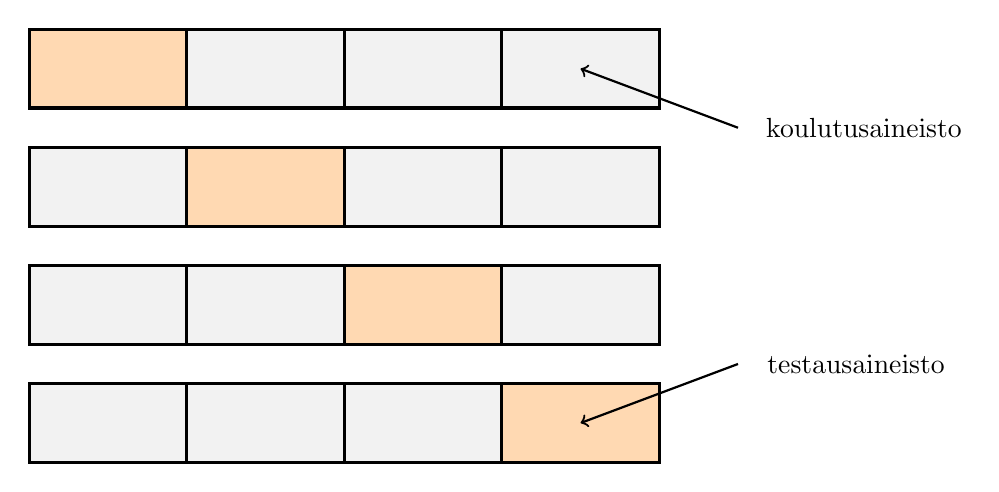
\begin{tikzpicture}
        \filldraw[color=black, fill=black!5, very thick] (0,0) rectangle (2,1);
        \filldraw[color=black, fill=black!5, very thick] (2,0) rectangle (4,1);
        \filldraw[color=black, fill=black!5, very thick] (4,0) rectangle (6,1);
        \filldraw[color=black, fill=orange!30, very thick] (6,0) rectangle (8,1);

        \filldraw[color=black, fill=black!5, very thick] (0,1.5) rectangle (2,2.5);
        \filldraw[color=black, fill=black!5, very thick] (2,1.5) rectangle (4,2.5);
        \filldraw[color=black, fill=orange!30, very thick] (4,1.5) rectangle (6,2.5);
        \filldraw[color=black, fill=black!5, very thick] (6,1.5) rectangle (8,2.5);

        \filldraw[color=black, fill=black!5, very thick] (0,3) rectangle (2,4);
        \filldraw[color=black, fill=orange!30, very thick] (2,3) rectangle (4,4);
        \filldraw[color=black, fill=black!5, very thick] (4,3) rectangle (6,4);
        \filldraw[color=black, fill=black!5, very thick] (6,3) rectangle (8,4);

        \filldraw[color=black, fill=orange!30, very thick] (0,4.5) rectangle (2,5.5);
        \filldraw[color=black, fill=black!5, very thick] (2,4.5) rectangle (4,5.5);
        \filldraw[color=black, fill=black!5, very thick] (4,4.5) rectangle (6,5.5);
        \filldraw[color=black, fill=black!5, very thick] (6,4.5) rectangle (8,5.5);

        \draw[thick, ->] (9,1.25) -- (7,0.5);
        \node[] at (10.5,1.25) {testausaineisto};

        \draw[thick, ->] (9,4.25) -- (7,5);
        \node[] at (10.6,4.25) {koulutusaineisto};
    \end{tikzpicture}
    \caption{Ristiinvalidoinnissa data-aineisto jaetaan kerrallaan $k$ osaan, missä $k-1$ osaa ovat koulutusaineistoa (harmaalla merkityt osuudet) ja yksi osa testausaineistoa (oranssilla merkitty osuus) \citep{deisenrothMathematicsMachineLearning2020}.}
\end{figure}

Koulutusaineistolla $\mathcal{R}$ koulutetun mallin $f$ suorituskykyä tarkastellaan testausaineiston $\mathcal{V}$ avulla, jolle lasketaan keskineliövirheen neliöjuuren avulla empiirinen riski testausaineistolla $\mathcal{V}$ \citep{deisenrothMathematicsMachineLearning2020}. K-kertaisessa ristiinvalidoinnissa lasketaan jokaiselle koulutusaineiston $k$-osan $\mathcal{R}^{(k)}$ predikaattorille $f^{(k)}$ empiirinen riski $R(f^{(k)}, \mathcal{V}^{(k)})$ käyttäen testiaineistoa $\mathcal{V}^{(k)}$. Kaikille mahdollisille $k$-osaan jaoille ristiinvalidointi arvioi odotetun yleistysvirheen kaavasta $$\mathds{E}_{\mathcal{V}}[R(f,\mathcal{V})] \approx \frac{1}{K}\sum^{K}_{k=1} R(f^{(k)}, \mathcal{V}^{(k)}).$$ Käytettävässä arvioinnissa on kaksi lähdettä, joista toisessa rajatulla koulutusaineistolla ei välttämättä saada parasta mahdollista $f^{(k)}$ ja toisessa testausaineistolla ei saada tarkkaa arviota riskistä $R(f^{(k)}, \mathcal{V}^{(k)})$.

\color{black}

\color{red}
Useiden eri mallien välisessä vertailussa naiivi Bayes oli ennustustamisen osalta paras algoritmi \citep{kotsiantisPREDICTINGSTUDENTSPERFORMANCE2004}.
\color{black}